\section{Implementation/Software} \label{sec:models}

The software implementation is illustrated with a reproducible
\proglang{Python} workflow based on the \pkg{fdfi} package. The example uses
the UCI Cardiotocography (CTG) data to demonstrate how the package handles
correlated predictors, fits a flow-based disentanglement model, computes
feature importance scores, and reports uncertainty diagnostics. Throughout
this section, functions, classes, and package components are marked using the
standard JSS conventions \code{code}, \class{class}, \fct{function}, and
\pkg{package}.

\subsection{Software organization}

The \pkg{fdfi} package is organized into three main layers. The module
\code{fdfi.models} implements the flow-matching model used to map the observed
feature space into an approximately independent latent space. The module
\code{fdfi.explainers} provides the user-facing attribution interface,
including the \class{FlowExplainer} class. The module \code{fdfi.utils}
implements reliability diagnostics and statistical utilities, while
\code{fdfi.plots} provides visualization helpers for correlation matrices,
importance summaries, and coefficient-of-variation diagnostics.

The notebook begins by importing the local package, installing notebook-only
plotting dependencies, and setting a fixed random seed for reproducibility.
The printed package version in the current notebook run is \code{0.0.5}.
%
\begin{Code}
%matplotlib inline

%pip install -q statsmodels adjustText

import sys
import os
sys.path.insert(0, os.path.abspath('..'))
import fdfi
print(fdfi.__version__)

from fdfi.explainers import FlowExplainer

import warnings
warnings.filterwarnings('ignore')

import numpy as np
import pandas as pd
import matplotlib.pyplot as plt
import matplotlib.patches as mpatches
from sklearn.ensemble import RandomForestClassifier
from sklearn.model_selection import train_test_split
from sklearn.metrics import accuracy_score, classification_report

RANDOM_STATE = 42
np.random.seed(RANDOM_STATE)
\end{Code}

\subsection{Data acquisition and pre-processing}

The CTG data are loaded directly from the UCI Machine Learning Repository. The
original spreadsheet contains non-data rows and additional columns, so the
notebook extracts the 21 predictor columns used in the analysis and the target
variable \code{NSP}. The target labels correspond to \emph{Normal},
\emph{Suspect}, and \emph{Pathological} fetal states.
%
\begin{Code}
CTG_URL = (
    'https://archive.ics.uci.edu/ml/machine-learning-databases/00193/CTG.xls'
)

raw = pd.read_excel(CTG_URL, sheet_name='Data', skiprows=1, header=0)
X_raw = raw.iloc[:, 10:31].copy()
y_raw = raw['NSP'].copy()

data = pd.concat([X_raw, y_raw], axis=1)

feature_names = [
    'LB', 'AC', 'FM', 'UC', 'DL', 'DS', 'DP', 'ASTV', 'MSTV', 'ALTV',
    'MLTV', 'Width', 'Min', 'Max', 'Nmax', 'Nzeros', 'Mode', 'Mean',
    'Median', 'Variance', 'Tendency'
]
data.columns = feature_names + ['NSP']

data = data.apply(pd.to_numeric, errors='coerce')
data.dropna(inplace=True)
data['NSP'] = data['NSP'].astype(int)

X = data[feature_names].values
y = data['NSP'].values
\end{Code}
%
This produces 2,126 complete observations with 21 predictors and one target
column. The empirical class distribution is shown in Table~\ref{tab:ctg-class}.

\begin{table}[t!]
\centering
\begin{tabular}{lrr}
\hline
Target class & Clinical label & Frequency \\ \hline
1 & Normal & 1655 \\
2 & Suspect & 295 \\
3 & Pathological & 176 \\ \hline
\end{tabular}
\caption{\label{tab:ctg-class} Class distribution of the cleaned CTG data.}
\end{table}

\subsection{Collinearity diagnostics}

Before fitting an attribution model, the notebook checks the empirical
correlation structure among CTG predictors. This step is important because
standard marginal perturbation schemes can be unreliable when predictors are
strongly dependent. The FHR summary statistics \code{Mean}, \code{Mode}, and
\code{Median} are expected to co-move, and the observed matrix confirms this.
%
\begin{Code}
from fdfi.plots import correlation_heatmap

fig, ax, feature_names_reordered = correlation_heatmap(
    X, feature_names,
    savepath='fig1_correlation_matrix.pdf'
)
plt.show()
\end{Code}
%
The three largest absolute pairwise correlations reported by the notebook are
shown in Table~\ref{tab:ctg-correlations}. Figure~\ref{fig:ctg-correlation}
shows the corresponding heatmap.

\begin{table}[t!]
\centering
\begin{tabular}{llr}
\hline
Feature 1 & Feature 2 & Absolute correlation \\ \hline
Mean & Median & 0.948251 \\
Mode & Median & 0.933399 \\
Width & Min & 0.898519 \\ \hline
\end{tabular}
\caption{\label{tab:ctg-correlations} Largest absolute pairwise correlations
in the original CTG feature matrix.}
\end{table}

\begin{figure}[t!]
\centering
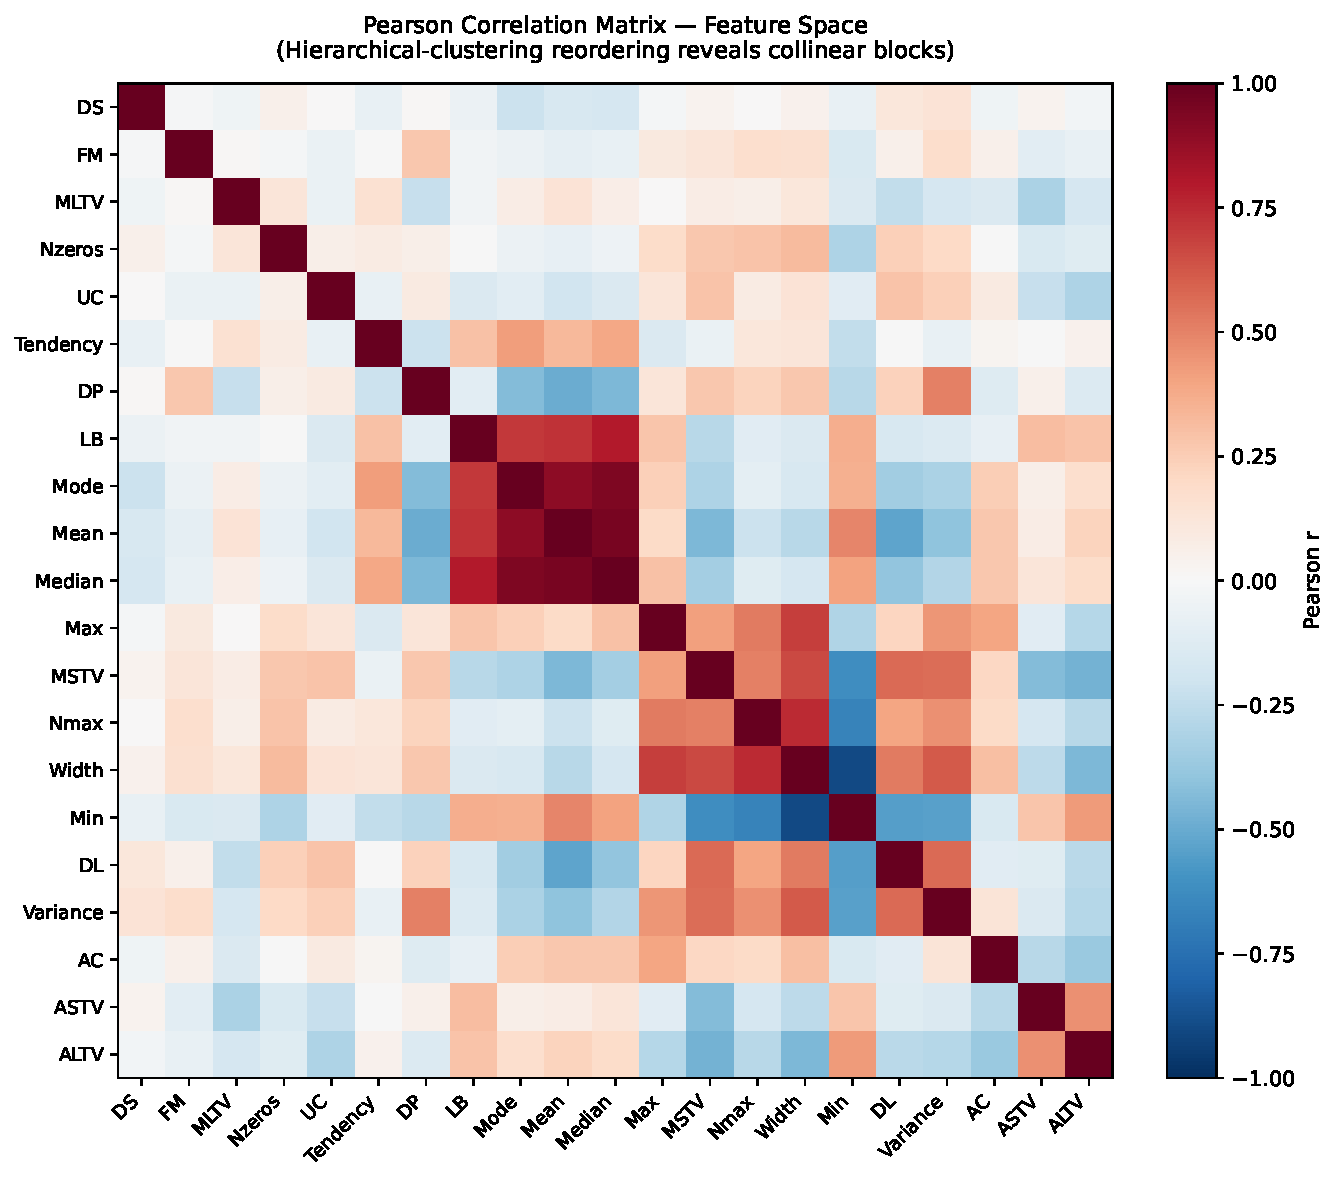
\includegraphics[width=0.92\textwidth]{img/fig1_correlation_matrix.pdf}
\caption{\label{fig:ctg-correlation} Correlation heatmap for the CTG
predictors. The strongest associations occur among fetal heart rate summary
statistics, motivating a disentanglement-based attribution method.}
\end{figure}

\subsection{Flow matching model}

The central object in \pkg{fdfi} is a learned transport from the correlated
feature space $\mathcal{X}$ to an approximately independent latent space
$\mathcal{Z}$,
%
\begin{equation} \label{eq:transport}
T_\theta: \mathcal{X} \longrightarrow \mathcal{Z}, \qquad
Z = T_\theta(X).
\end{equation}
%
The package implements this map using a continuous normalizing flow trained by
Flow Matching. Let $x_0 \sim \mathcal{N}(0, I)$ denote a Gaussian source sample
and let $x_1 \sim p(X)$ denote an observed data sample. The straight-path
interpolant is
%
\begin{equation} \label{eq:path}
x_t = (1 - (1 - \sigma_{\min})t)x_0 + t x_1.
\end{equation}
%
The velocity field $v_\theta(x,t)$ is trained by minimizing
%
\begin{equation} \label{eq:flow-loss}
\mathcal{L}(\theta) =
\E_{t,x_0,x_1}
\left[
\left\|
v_\theta(x_t,t) -
\{x_1 - (1 - \sigma_{\min})x_0\}
\right\|^2
\right].
\end{equation}
%
At inference time, the learned ODE is integrated forward or backward to obtain
$T_\theta$ and $T_\theta^{-1}$.

\begin{table}[t!]
\centering
\small
\begin{tabular}{p{2.5cm}p{1.7cm}p{1.6cm}p{6.2cm}}
\hline
Parameter & Type & Default & Description \\ \hline
\code{X} & array & -- & Training data defining the target distribution $p(X)$. \\
\code{dim} & integer & -- & Feature dimensionality $d$. \\
\code{hidden\_dim} & integer & 64 & Width of each residual MLP block. \\
\code{time\_embed\_dim} & integer & 32 & Dimension of the sinusoidal time embedding. \\
\code{num\_blocks} & integer & 1 & Number of residual MLP blocks in the trunk. \\
\code{sigma\_min} & numeric & 0.01 & Path-noise floor preventing degeneracy near $t=0$. \\
\code{num\_steps} & integer & 5000 & Number of training iterations passed to \fct{fit}. \\
\code{verbose} & logical/string & final & Controls training output verbosity. \\ \hline
\end{tabular}
\caption{\label{tab:flow-parameters} Key constructor and fitting parameters
for \class{FlowMatchingModel}.}
\end{table}

\subsection{Feature attribution interface}

Given a trained flow, the \class{FlowExplainer} class implements the complete
FDFI attribution pipeline. The explainer is initialized with a model callable
and background data. Importance scores are then obtained by calling the
explainer on a matrix of test observations.

For each feature $j$ and test point $x^{(i)}$, the explainer constructs
counterfactual samples by encoding $x^{(i)}$ to
$z^{(i)} = T_\theta(x^{(i)})$, replacing the $j$th latent coordinate, and
decoding the modified latent sample back to feature space. The conditional
permutation importance used in the notebook is
%
\begin{equation} \label{eq:cpi}
\phi_j^{\mathrm{CPI}}(x^{(i)}) =
\left(
f(x^{(i)}) -
\frac{1}{B}\sum_{b=1}^{B} f(\tilde{x}^{(i,b)})
\right)^2,
\end{equation}
%
where $B$ is controlled by the argument \code{nsamples} and
$\tilde{x}^{(i,b)}$ denotes a decoded counterfactual copy. The Sobol-CPI
alternative is
%
\begin{equation} \label{eq:scpi}
\phi_j^{\mathrm{SCPI}}(x^{(i)}) =
\mathrm{Var}_b\{f(\tilde{x}^{(i,b)})\}.
\end{equation}
%
Importance is projected back to the original feature space using the decoder
Jacobian $H = \partial X / \partial Z$,
%
\begin{equation} \label{eq:back-projection}
\phi_l^X = \sum_{k=1}^d H_{lk}^2 \phi_k^Z,
\qquad l = 1,\ldots,d.
\end{equation}

\begin{table}[t!]
\centering
\small
\begin{tabular}{p{2.9cm}p{1.9cm}p{7.1cm}}
\hline
Argument or output & Role & Description \\ \hline
\code{nsamples} & Attribution & Monte Carlo draws per feature and sample. \\
\code{method} & Attribution & \code{cpi}, \code{scpi}, or \code{both}. \\
\code{sampling\_method} & Attribution & One of \code{resample}, \code{permutation}, \code{normal}, or \code{condperm}. \\
\code{phi\_X} & Output & Mean importance in the original feature space. \\
\code{se\_X} & Output & Bootstrap standard error of \code{phi\_X}. \\
\code{alpha} & Inference & Nominal type-I error rate for confidence intervals. \\
\code{var\_floor\_method} & Inference & Variance-floor adjustment, e.g., \code{mixture} or \code{fixed}. \\
\code{groups} & Inference & Optional feature groups passed to \fct{conf\_int}. \\
\code{multitest\_method} & Inference & Multiple-testing correction, e.g., \code{fdr\_bh}, \code{bonferroni}, or \code{holm}. \\
\code{score} & Output & Feature-level or group-level importance estimate returned by \fct{conf\_int}. \\
\code{pvalue\_adj} & Output & Multiple-testing adjusted $p$ values. \\ \hline
\end{tabular}
\caption{\label{tab:flow-explainer-api} Main arguments and outputs used by
\class{FlowExplainer} and \fct{conf\_int}.}
\end{table}

\subsection{Reliability metrics}

The \pkg{fdfi} workflow includes a self-certification stage before attribution
scores are interpreted. The first diagnostic is the Maximum Mean Discrepancy
(MMD) between the original feature distribution and the reconstructed
distribution. Using a Gaussian RBF kernel $k(\cdot,\cdot)$,
%
\begin{equation} \label{eq:mmd}
\mathrm{MMD}^2(p,q) =
\E_{x,x' \sim p}\{k(x,x')\}
+ \E_{z,z' \sim q}\{k(z,z')\}
- 2\E_{x \sim p,z \sim q}\{k(x,z)\}.
\end{equation}
%
The second diagnostic is the median off-diagonal distance correlation among
latent coordinates. If $\mathcal{V}^2$ denotes distance covariance, then
%
\begin{equation} \label{eq:dcor}
\mathrm{dCor}(Z_j,Z_k) =
\frac{\mathcal{V}^2(Z_j,Z_k)}
{\sqrt{\mathcal{V}^2(Z_j,Z_j)\mathcal{V}^2(Z_k,Z_k)}}.
\end{equation}
%
The scalar diagnostic reported by the package is
%
\begin{equation} \label{eq:median-dcor}
\widetilde{\mathrm{dCor}} =
\underset{j \ne k}{\mathrm{median}}\,\mathrm{dCor}(Z_j,Z_k).
\end{equation}

\begin{table}[t!]
\centering
\small
\begin{tabular}{p{3.1cm}p{4.0cm}lll}
\hline
Diagnostic & Key & GOOD & MODERATE & POOR \\ \hline
Latent independence & \code{latent\_independence\_median} &
$<0.10$ & $[0.10,0.25)$ & $\geq 0.25$ \\
Distribution fidelity & \code{distribution\_fidelity\_mmd} &
$<0.05$ & $[0.05,0.15)$ & $\geq 0.15$ \\ \hline
\end{tabular}
\caption{\label{tab:diagnostic-thresholds} Qualitative thresholds for
\pkg{fdfi} reliability diagnostics. Lower values are better for both metrics.}
\end{table}

\begin{table}[t!]
\centering
\small
\begin{tabular}{p{4.2cm}p{2.1cm}p{6.1cm}}
\hline
Method or attribute & Returns & Description \\ \hline
\code{explainer.diagnostics} & dictionary & Automatically populated during initialization. \\
\fct{explainer.diagnose} & dictionary & Re-runs diagnostics on demand. \\
\code{explainer.diagnostics['latent\_independence\_dcor']} &
array & Full pairwise distance-correlation matrix. \\ \hline
\end{tabular}
\caption{\label{tab:diagnostic-accessors} Accessor interface for diagnostics
in \pkg{fdfi}.}
\end{table}

\subsection{Black-box classifier}

FDFI is model-agnostic. In the CTG example, the notebook uses a random forest
classifier as the predictive model $f$. The data are stratified into training
and test sets, standardized, and then fitted with
\class{RandomForestClassifier}.
%
\begin{Code}
from sklearn.preprocessing import StandardScaler

X_train, X_test, y_train, y_test = train_test_split(
    X, y, test_size=0.20, random_state=RANDOM_STATE, stratify=y
)

scaler = StandardScaler()
X_train = scaler.fit_transform(X_train)
X_test = scaler.transform(X_test)

model = RandomForestClassifier(
    n_estimators=300,
    max_depth=None,
    min_samples_leaf=2,
    n_jobs=-1,
    random_state=RANDOM_STATE,
)
model.fit(X_train, y_train)

y_pred = model.predict(X_test)
acc = accuracy_score(y_test, y_pred)
\end{Code}
%
The held-out accuracy is $0.9225$ on 426 test samples. Class-wise performance
is summarized in Table~\ref{tab:classification-report}.

\begin{table}[t!]
\centering
\begin{tabular}{lrrrr}
\hline
Class & Precision & Recall & F1 score & Support \\ \hline
Normal (1) & 0.93 & 0.98 & 0.96 & 332 \\
Suspect (2) & 0.86 & 0.61 & 0.71 & 59 \\
Pathological (3) & 0.91 & 0.86 & 0.88 & 35 \\
Macro average & 0.90 & 0.82 & 0.85 & 426 \\
Weighted average & 0.92 & 0.92 & 0.92 & 426 \\ \hline
\end{tabular}
\caption{\label{tab:classification-report} Test-set classification report for
the random forest model. Overall accuracy is 0.9225.}
\end{table}

\subsection{Flow diagnostics in the CTG example}

The predictive model is wrapped to return the probability of the pathological
class. The \class{FlowExplainer} is then initialized with the standardized
training data and \code{nsamples = 50}.
%
\begin{Code}
def model_wrapper(X):
    return model.predict_proba(X)[:, 2]

explainer = FlowExplainer(
    model_wrapper,
    X_train,
    nsamples=50,
)

diag = explainer.diagnostics
mmd_val = diag['distribution_fidelity_mmd']
dcor_val = diag['latent_independence_median']
\end{Code}
%
The flow was trained for 5,000 steps with final loss 1.0836. The diagnostic
values are reported in Table~\ref{tab:ctg-diagnostics}. Both pass the
recommended thresholds in Table~\ref{tab:diagnostic-thresholds}.

\begin{table}[t!]
\centering
\begin{tabular}{llll}
\hline
Diagnostic & Value & Threshold & Result \\ \hline
Distribution fidelity, MMD & 0.029164 & $<0.05$ & PASS \\
Latent independence, median dCor & 0.092052 & $<0.10$ & PASS \\ \hline
\end{tabular}
\caption{\label{tab:ctg-diagnostics} Flow diagnostics for the CTG run.}
\end{table}

\subsection{Feature attribution and visualisation}

The notebook computes FDFI attributions for 100 held-out test observations.
The returned arrays \code{phi\_X} and \code{se\_X} are aggregated to obtain
global importance scores and standard errors.
%
\begin{Code}
N_EXPLAIN = 100
X_explain = X_test[:N_EXPLAIN]

results = explainer(X_explain)

phi_X = results['phi_X']
se_X = results['se_X']

if phi_X.ndim == 2:
    global_phi = np.abs(phi_X).mean(axis=0)
    global_se = se_X.mean(axis=0)
else:
    global_phi = np.abs(phi_X)
    global_se = se_X

importance_df = (
    pd.DataFrame({'feature': feature_names, 'phi': global_phi, 'se': global_se})
    .sort_values('phi', ascending=False)
    .reset_index(drop=True)
)

_ = explainer.summary(
    alpha=0.05,
    target='X',
    alternative='greater',
    multitest_method='fdr_bh',
)
\end{Code}
%
The standardized inference summary in this run reports 21 units, a one-sided
alternative, Benjamini-Hochberg FDR adjustment, and no rejected feature-level
null hypotheses at $\alpha = 0.05$. Selected output values are shown in
Table~\ref{tab:feature-summary}.

\begin{table}[t!]
\centering
\begin{tabular}{rrrrrr}
\hline
Feature index & Estimate & Std. err. & CI lower & CI upper & Adjusted $p$ \\ \hline
0 & 0.0056 & 0.0038 & -0.0007 & $\infty$ & 0.3946 \\
1 & 0.0039 & 0.0035 & -0.0018 & $\infty$ & 0.3946 \\
3 & 0.0044 & 0.0037 & -0.0017 & $\infty$ & 0.3946 \\
7 & 0.0068 & 0.0046 & -0.0009 & $\infty$ & 0.3946 \\
18 & 0.0058 & 0.0039 & -0.0006 & $\infty$ & 0.3946 \\
20 & 0.0036 & 0.0036 & -0.0022 & $\infty$ & 0.4106 \\ \hline
\end{tabular}
\caption{\label{tab:feature-summary} Selected rows from the standardized
feature-level inference summary. No feature-level null hypothesis is rejected
after FDR adjustment at $\alpha = 0.05$.}
\end{table}

The global importance bar chart is generated with \fct{summary\_bar}. The
notebook colors features by clinically meaningful groups.
%
\begin{Code}
from fdfi.plots import summary_bar

GROUP_COLOUR = {
    'LB': '#4878a8', 'ASTV': '#4878a8', 'MSTV': '#4878a8',
    'ALTV': '#4878a8', 'MLTV': '#4878a8', 'Variance': '#4878a8',
    'AC': '#e07b54', 'FM': '#e07b54', 'UC': '#e07b54',
    'DL': '#e07b54', 'DS': '#e07b54', 'DP': '#e07b54',
    'Width': '#3a9e8c', 'Min': '#3a9e8c', 'Max': '#3a9e8c',
    'Nmax': '#3a9e8c', 'Nzeros': '#3a9e8c', 'Tendency': '#3a9e8c',
    'Mode': '#c9a227', 'Mean': '#c9a227', 'Median': '#c9a227',
}

fig, ax, importance_df_sorted = summary_bar(
    global_phi, global_se, feature_names,
    group_colors=GROUP_COLOUR,
    savepath='fig2_fdfi_importance.pdf'
)
plt.show()
\end{Code}

\begin{figure}[t!]
\centering
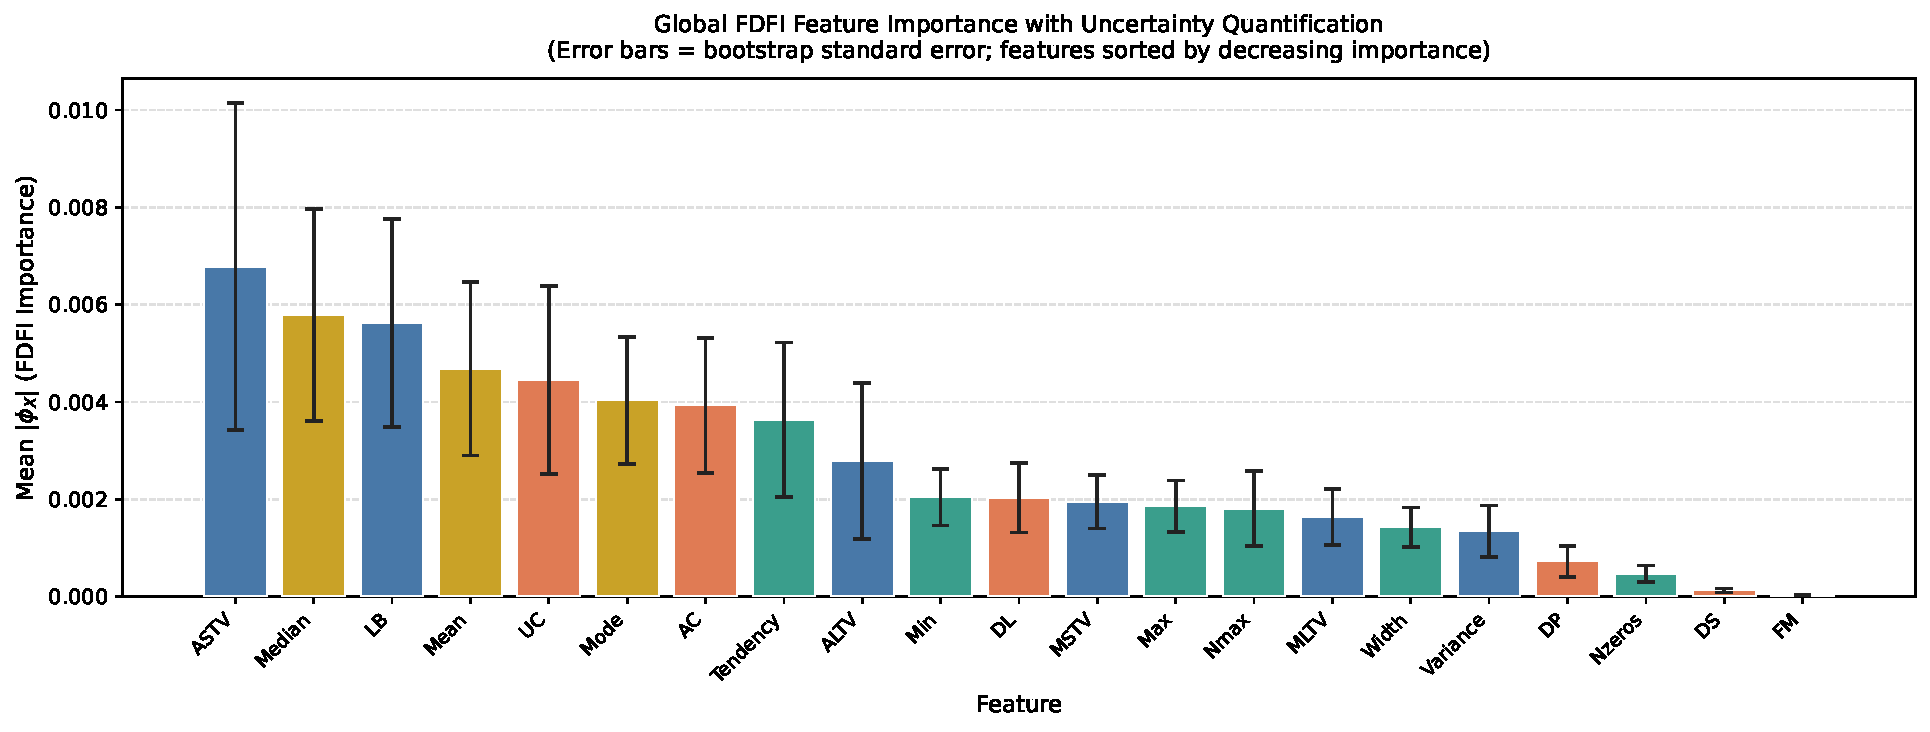
\includegraphics[width=0.92\textwidth]{img/fig2_fdfi_importance.pdf}
\caption{\label{fig:ctg-importance} Global FDFI importance estimates for the
CTG example, with uncertainty bars based on bootstrap standard errors returned
by \class{FlowExplainer}.}
\end{figure}

\subsection{Group-level clinical inference}

The current \pkg{fdfi} API also supports grouped inference through
\fct{conf\_int}. In the CTG example, predictors are grouped into four clinical
families: FHR baseline and variability, accelerations and decelerations,
histogram morphology, and FHR central tendency.
%
\begin{Code}
clinical_groups = {
    'FHR baseline & variability': [
        feature_names.index(f)
        for f in ['LB', 'ASTV', 'MSTV', 'ALTV', 'MLTV', 'Variance']
    ],
    'Accelerations & decelerations': [
        feature_names.index(f)
        for f in ['AC', 'FM', 'UC', 'DL', 'DS', 'DP']
    ],
    'Histogram morphology': [
        feature_names.index(f)
        for f in ['Width', 'Min', 'Max', 'Nmax', 'Nzeros', 'Tendency']
    ],
    'FHR central tendency': [
        feature_names.index(f)
        for f in ['Mode', 'Mean', 'Median']
    ],
}

group_ci = explainer.conf_int(
    alpha=0.05,
    target='X',
    alternative='greater',
    groups=clinical_groups,
    multitest_method='fdr_bh',
)

group_ci_df = (
    pd.DataFrame({
        'group': group_ci['groups'],
        'score': group_ci['score'],
        'se': group_ci['se'],
        'ci_lower': group_ci['ci_lower'],
        'pvalue': group_ci['pvalue'],
        'pvalue_adj': group_ci['pvalue_adj'],
        'reject_fdr': group_ci['reject_null'],
    })
    .sort_values('score', ascending=False)
    .reset_index(drop=True)
)
\end{Code}
%
The resulting grouped inference table is shown in
Table~\ref{tab:group-inference}. No group is rejected after FDR adjustment at
the 5 percent level.

\begin{table}[t!]
\centering
\small
\begin{tabular}{p{4.0cm}rrrrr}
\hline
Group & Score & SE & CI lower & Adjusted $p$ & Reject FDR \\ \hline
FHR baseline and variability & 0.020109 & 0.009590 & 0.004335 & 0.669968 & False \\
FHR central tendency & 0.014491 & 0.008333 & 0.000784 & 0.669968 & False \\
Accelerations and decelerations & 0.011276 & 0.007346 & -0.000807 & 0.669968 & False \\
Histogram morphology & 0.011225 & 0.007425 & -0.000988 & 0.669968 & False \\ \hline
\end{tabular}
\caption{\label{tab:group-inference} Group-level clinical inference from
\fct{conf\_int} using FDR-adjusted $p$ values.}
\end{table}

\subsection{Coefficient-of-variation diagnostics}

The notebook further examines attribution reliability using the coefficient of
variation
%
\begin{equation} \label{eq:cv}
\mathrm{CV}_j = \frac{\mathrm{se}_j}{\phi_j}.
\end{equation}
%
The robust standard errors are extracted from \fct{conf\_int}, which applies
the variance-floor and margin adjustments used by the inference routine.
%
\begin{Code}
from fdfi.plots import cv_scatter

ci_df = explainer.conf_int(
    alpha=0.05,
    target='X',
    alternative='greater',
    multitest_method='fdr_bh',
)

enlarged_se = _extract_enlarged_se(ci_df, n_features=len(feature_names))

fig, ax, cv_df_filtered, cv_df_outliers = cv_scatter(
    global_phi,
    enlarged_se,
    feature_names,
    y_cutoff=3.0,
    group_colors=GROUP_COLOUR,
    figsize=(11.5, 4.0),
)

fig.savefig('fig3_cv_scatter.pdf', bbox_inches='tight')
plt.show()
\end{Code}
%
The mean raw standard error is 0.001070, while the mean enlarged standard error
is 0.003460. The notebook reports 17 displayed features with
$\mathrm{CV} \leq 3.0$ and four high-CV features, namely \code{DP},
\code{Nzeros}, \code{DS}, and \code{FM}. Figure~\ref{fig:ctg-cv} shows the
coefficient-of-variation diagnostic.

\begin{figure}[t!]
\centering

\includegraphics[width=0.92\textwidth]{img/fig3_cv_scatter.pdf}
\caption{\label{fig:ctg-cv} Coefficient-of-variation diagnostic for the CTG
importance estimates. Features above the reference line have uncertainty larger
than their point estimate; features with CV greater than 3 are capped in the
display.}
\end{figure}

\subsection{Sampling methods in latent space}

The final notebook section compares three latent-space sampling strategies:
\code{resample}, \code{permutation}, and \code{normal}. This comparison uses
20 held-out test observations and re-initializes \class{FlowExplainer} for
each sampling method.
%
\begin{Code}
N_DEMO = 20
X_demo = X_test[:N_DEMO]

sampling_methods = ['resample', 'permutation', 'normal']
results_by_method = {}

for method in sampling_methods:
    explainer_sm = FlowExplainer(
        model_wrapper,
        X_train,
        sampling_method=method,
        nsamples=50,
    )
    results_by_method[method] = explainer_sm(X_demo)
\end{Code}
%
The resulting feature-importance comparison is summarized in
Table~\ref{tab:sampling-methods}. The largest magnitudes occur for the
variability-related features \code{ALTV}, \code{ASTV}, and \code{MSTV}, and
the broad ranking pattern is stable across counterfactual sampling schemes.

\begin{table}[t!]
\centering
\begin{tabular}{lrrr}
\hline
Feature & Resample & Permutation & Normal \\ \hline
LB & 0.000174 & 0.000095 & 0.000272 \\
AC & 0.000290 & 0.000131 & 0.000241 \\
FM & 0.000001 & 0.000000 & 0.000001 \\
UC & 0.000100 & 0.000054 & 0.000082 \\
DL & 0.000244 & 0.000227 & 0.000350 \\
DS & 0.000001 & 0.000000 & 0.000001 \\
DP & 0.000003 & 0.000000 & 0.000048 \\
ASTV & 0.000655 & 0.000239 & 0.000687 \\
MSTV & 0.000618 & 0.000726 & 0.000718 \\
ALTV & 0.001523 & 0.000174 & 0.000989 \\
MLTV & 0.000072 & 0.000067 & 0.000056 \\
Width & 0.000145 & 0.000110 & 0.000158 \\
Min & 0.000150 & 0.000121 & 0.000184 \\
Max & 0.000082 & 0.000067 & 0.000117 \\
Nmax & 0.000079 & 0.000072 & 0.000083 \\
Nzeros & 0.000120 & 0.000090 & 0.000119 \\
Mode & 0.000088 & 0.000086 & 0.000220 \\
Mean & 0.000147 & 0.000172 & 0.000337 \\
Median & 0.000113 & 0.000101 & 0.000307 \\
Variance & 0.000103 & 0.000082 & 0.000116 \\
Tendency & 0.000026 & 0.000023 & 0.000040 \\ \hline
\end{tabular}
\caption{\label{tab:sampling-methods} Feature importance comparison across
latent-space sampling methods on 20 held-out CTG observations.}
\end{table}

\subsection{Summary of the implementation workflow}

The CTG example demonstrates the complete \pkg{fdfi} workflow: data loading and
cleaning, collinearity diagnosis, black-box model training, flow-based
disentanglement, reliability checking, feature-level attribution,
group-level inference, and sampling-method comparison. The key implementation
point is that attribution is not reported in isolation. Each explanation is
paired with diagnostics for distribution fidelity and latent independence, as
well as standard errors, confidence bounds, and multiple-testing adjusted
inference summaries.
